\documentclass[conference]{IEEEtran}

\usepackage[utf8]{inputenc}
\usepackage[
    margin=1in,
    includehead,
    %includefoot,
]{geometry}

% ---------------------------------------

\usepackage{indentfirst}
\usepackage{cite}
\usepackage{amsmath, amssymb, amsfonts}
\usepackage{color, colortbl}
\usepackage{graphicx}
\usepackage[table]{xcolor}
\usepackage{siunitx}
\usepackage{algorithm, algpseudocode}
\usepackage{placeins}

% ---------------------------------------

\usepackage{makecell}
\renewcommand\theadalign{bc}
\renewcommand\theadfont{\bfseries}
\renewcommand\theadgape{\Gape[4pt]}
\renewcommand\cellgape{\Gape[4pt]}

% ---------------------------------------

\usepackage{fancyhdr}
\pagestyle{fancy}
\fancyhf{}
%\renewcommand{\headrulewidth}{0pt}
\fancyhead[L]{Page \thepage}
\fancyhead[R]{Predicting Stock Market Trends}

% ---------------------------------------

\title{CSCI 4/5850-001 Team 5\\Predicting Stock Market Trends}
\author{
    \IEEEauthorblockN{Devin Jean}
    \IEEEauthorblockA{
    \textit{Computer Science Department} \\
    \textit{Middle Tennessee State University}\\
    Murfreesboro, USA \\
    dcj2z@mtmail.mtsu.edu
    }
    \and
    \IEEEauthorblockN{Jie Long}
    \IEEEauthorblockA{
    \textit{Computer Science Department} \\
    \textit{Middle Tennessee State University}\\
    Murfreesboro, USA \\
    jl7u@mtmail.mtsu.edu
    }
    \and
    \IEEEauthorblockN{Hunter McGee}
    \IEEEauthorblockA{
    \textit{Computer Science Department} \\
    \textit{Middle Tennessee State University}\\
    Murfreesboro, USA \\
    hkm3c@mtmail.mtsu.edu
    }
    \and
    \IEEEauthorblockN{Ryan Morse}
    \IEEEauthorblockA{
    \textit{Computer Science Department} \\
    \textit{Middle Tennessee State University}\\
    Murfreesboro, USA \\
    rjm5q@mtmail.mtsu.edu
    }
    \and
    \IEEEauthorblockN{Paul Myers}
    \IEEEauthorblockA{
    \textit{Computer Science Department} \\
    \textit{Middle Tennessee State University}\\
    Murfreesboro, USA \\
    pim2b@mtmail.mtsu.edu
    }
    \and
    \IEEEauthorblockN{Thomas Torku}
    \IEEEauthorblockA{
    \textit{University Studies Department} \\
    \textit{Middle Tennessee State University}\\
    Murfreesboro, USA \\
    thomas.torku@mtsu.edu
    }
}

\begin{document}
\maketitle
\thispagestyle{empty}

\begin{abstract}
The chaotic nature of the stock market and the potential profit has intrigued many gambling eyes.
How can we predict something that's so unpredictable?
Through the advancement in Neural Networks, we can attempt to solve this question with multiple different types of Neural Nets such as DNNs or LSTM nets.
The focus of this study is to compare each model to traditional regressive models for predicting stocks, such as ARIMA.
Yahoo! Finance offers a plethora of market data, with which we attempted to compare four stocks: IXIC, N225, DJI, and GSPC.
To compare these different models' accuracies, we used \textit{Root Mean Square Error (RMSE)} as our error metric.
After analyzing our benchmarking results, we have come to the conclusion that although neural networks have the potential to outperform traditional regressive models such as ARIMA, we failed to create one that shows this.
\end{abstract}
\begin{IEEEkeywords}
Neural Networks, ARIMA, Time Series, RMSE, DNN
\end{IEEEkeywords}

\section{Introduction}

The volatility of the market demands a very robust approach to predicting stock prices even when only projecting one day into the future.
Moreover, the data used in the modelling process is almost always noisy due to unknown or even unknowable variables such as political shifts and natural disasters \cite{torku2016takens}.
Classical approaches are primarily regression-based.
Although extensively used, they have many limitations in application; for instance, their assumptions of linearity and normality are but a few examples of potential shortcomings \cite{siami2018forecasting, torku2016takens}.
The most popular classical regression technique used is \textit{Autoregressive Integrated Moving Averages (ARIMA)}, which can be applied to both univariate and multivariate time series data and can produce good results in terms of prediction accuracy and errors.

The evolution of data science, machine learning, and deep learning has led to the development of many methods which produce even better results than ARIMA.
Among the many machine-learning tools used are Support Vector Machines (SVM) and Random Forests (RF).
Similarly, the deep learning neural networks tools include Deep Neural Networks (DNN), Convolution Neural Networks (CNN), Long Short-Term Memory (LSTM), and Deep Belief Networks (DBN).
In this work, we focused on DNN and LSTM.
Our work compares the results from these networks regarding the prediction of the closing price of four stocks.

\section{Background}

As a time series problem, the input to any of these methods would be some (typically contiguous) sequence of time point values, and the output would be the predicted value for a future time point.
For most models, this can be easily extended to map many concurrent time sequences into many simultaneous predictions.

However, aside from these similarities most models are quite different in their approach to predictions:

\subsection{DNN Model}
One of the prevailing difficulties in stock market analysis is that it's chaotic; although not completely random, there are so many complex nonlinear relationships between so many variables that it appears to be random even upon many forms of regressive analysis \cite{lawrence}.
However, deep learning is theoretically capable of learning some of these types of decision boundaries.
Therefore, given a sufficient sampling of the market for many stocks, the hope is that the network will have enough information to cut through the chaos and be able to predict market trends in a much better way than traditional techniques \cite{lawrence}.

In this paper, what we refer to as the \textit{Deep Neural Network (DNN)} model is a traditional feed-forward net which is not armed with any other form of inductive bias.
It simply receives the input and maps it through its layers in a single pass with dense connections from one layer to the next.

\subsection{ARIMA Model}
\subsubsection{Autoregressive Model}
Autoregressive models make full use of the dependencies between several lagged observations and an observation \cite{tsay, pesaran2015time}.
A model of finite order $p \in \mathbb{N}$ is written as
\begin{align}
    x_t &= \phi_0 + \phi_1 x_{t-1} + \phi_2 x_{t-2} + \dots + \phi_p x_{t-p} + \epsilon_t \\
    &= \phi_0 + \epsilon_t + \sum_{i=1}^p{\phi_i x_{t-i}}
\end{align}
where $\phi_0$ is a positive number, $\phi_{1...p}$ are autocorrelation coefficients, $\epsilon$ is a Gaussian white noise time series, a sequence of random numbers with mean 0 and variance $\sigma^2$, $x_t$ are stationary random variables, and $x_{t-p}$ are the first $p$ lagged variables.
This equation could be explained as the conditioned expectation of $x_{t}$ as determined by the past values $x_{1...t-1}$ \cite{tsay}.

\subsubsection{Moving Average Model}
The \textit{Moving Average (MA)} model is an infinite-order AR model, with some parameter constraints, and is constructed as
\begin{align}
    x_t &= \mu + \epsilon_t + \theta_1\epsilon_{t-1} + \dots + \theta_q\epsilon_{t-q} \\
    &= \mu + \epsilon_t + \sum_{i=1}^q{\theta_i \epsilon_{t-i}}
\end{align}
where $\mu$ is the expectation of series $x_t$, $\epsilon$ is the Gaussian white noise series, and $\theta$ are the parameters of the model with $\theta_0 \equiv 1$ \cite{tsay}.

\subsubsection{Autoregressive Moving Average Model}
The ARMA($p, q$) model is a combination of the AR($p$) and MA($q$) models (order in parenthesis).
The model is written as
\begin{equation}
    x_t = \phi_0 + \left(\sum_{i=1}^p{\phi_i x_{t-i}}\right) + \epsilon_t + \left(\sum_{i=0}^q{\theta_i \epsilon_{t-i}}\right)
\end{equation}
where the $\epsilon_{t}$ is the white noise series - the time series with finite mean value and variance $\sigma^2$ \cite{tsay}.
In order to maintain the usefulness of this model, we assert that $\forall i \enspace \phi_i \ne \theta_i$ because their equivalence would result in a lost degree of freedom.

\subsubsection{Autoregressive Integrated Moving Average Model}
The general form of the ARIMA model is ARIMA($p, d, q$).
Here, the "I" denotes "integrated", which makes the time series stationary by replacing the data value with the difference between their values and the previous values.
Identifying the values of $p$, $d$ and $q$ is an important step in constructing an ARIMA model.

Firstly, the $p$ value can be determined by the \textit{autocorrelation function (ACF)}.
The ACF of $x_t$ is the collection of lag-$k$ autocorrelations $\rho_k$, which is the correlation coefficient between $x_t$ and $x_{t-k}$.
The $q$ value is then determined by the \textit{partial autocorrelation function (PACF)}, which is a function of the stationary time series' ACF.
Lastly, the $d$ value is the order of difference frequency in the conversion from non-stationary to stationary time series \cite{tsay}.

Once these values are computed, they can simply be substituted into the relevant equations to calculate the predicted values from ARIMA analysis.

\subsection{LSTM Model}
The \textit{Long Short-Term Memory (LSTM)} model is a deep neural network that contains LSTM cells in the hidden (computational) layers of the network \cite{brownlee2016time}.
LSTM cells differ from normal neurons in that they have a form of self-connection that allows them to hold an internal state.
This is typically referred to as the cell's memory.
There are also other parts of the cell that control how, when, and what it forgets - all of which is learned by the network during training.

This sort of network architecture is typically used for a problem where the inputs are given in discrete quanta one by one as a sequence, and the network folds them all together into the final answer at the end of the input sequence.
Thus, this is potentially a very promising model for learning time-series data, as the folding of stock data might allow us to learn the market's intrinsic characteristic of chronological causality.
For example, a dip in a stock might have implications for what happens in the next time step, and so on \cite{olah2015understanding}.

\subsection{DBN Model}
The \textit{Deep Belief Network (DBN)} model is a deep neural network that consists of an input layer with many hidden layers laid out sequentially before reaching an output layer much like a \textit{Multilayer Perceptron (MLP)}; however, there are a few key differences between a DBN versus a MLP.
First, it is helpful to understand the key component of the DBN architecture: \textit{Restricted Boltzmann Machines (RBM)}.

A Restricted Boltzmann Machine is a 2-layer network where the first layer is the visible layer and the second layer is the hidden layer.
The two layers are connected via undirected edges, where a node in one layer is connected \textit{only} to all the nodes in the other layer.
An RBM is trained through a sequence of forward and backward passes to encode a representation of the data and then reconstruct the input data\cite{hinton}.
Because of this method of training, an RBM is effective at extracting relevant features from the data.

The DBN can be thought of as a sequential stack of these Restricted Boltzmann Machines, where the hidden layer of the preceding RBM feeds into the next.
The hidden layer of the last RBM then feeds in to a single output layer.
Because of the training nature of an RBM, we can pretrain each RBM in an unsupervised manner before starting any backpropagation throughout the whole network.
The pretrained RBM's are then used to initialize the weights of the network \cite{NIPS2006}.
Since the RBMs have attempted to reconstruct the input to some level of precision, some internal representation has been formed.
This leads to "more effective" initialized weights than ones that are randomly generated -- hence increasing speed of convergence in the supervised training phase (backpropagation).

\section{Methods}

\subsection{Data Preparation}
In order to facilitate the collection of stock data used in this project we used \texttt{yfinance}, a python API that queries Yahoo! Finance \cite{yfinanceapi}.
For reproducibility and benchmarking purposes, the start and stop dates for data fetching are constant: 1/1/1985 -- 8/1/2018.
The following stocks/indices were used: Nasdaq (IXIC), DJI (Dow Jones), GSPC (S\&P 500), and Nikkei 225.
These stocks were selected to give detailed information about several large companies, as well as two indices (DJI and GSPC) to give summarized context for many other stocks that were not considered explicitly.

From this raw daily stock data, we considered overlapping windows of size 200 for input, and took the following day (one time point in the future) as the expected value for the prediction.
The value 200 was chosen arbitrarily, but is believed to be sufficiently large to provide enough information for any given model to be able to decode recent market trends.
Each of these input-output pairs was then normalized by dividing by the first (oldest) time point in the input for each stock.
This resulted in the first input for any stock always being 1 and all other inputs and outputs being multiplicatively relative to it.
This strategy was done to normalize against the effects of stocks with vastly different values so that the network can learn the percent increase/decrease trends rather than the values of stocks themselves.

\subsection{Modeling}
For this analysis, we have constructed models for the LSTM, DNN, and ARIMA approaches to market prediction.
The data obtained from Yahoo! finance was split 70-30 into training and testing sets respectively.
This was done to guard against false positives in predictive accuracy due to overfitting.

The rolling forecast approach was used for ARIMA, which folds previous data points to predict future data points \cite{hyndman2018forecasting}.
The models were built and run in python.
The Keras and Tensorflow frameworks were utilized for deep learning models.
The \textit{Mean Squared Error (MSE)} loss function and the Adam optimizer were used for the DNN and LSTM models.
Algorithm~\ref{alg:model} represents the general logical structure for testing each model.
\begin{algorithm}[ht]
\begin{algorithmic}[1]
    \caption{For LSTM, DNN and ARIMA Models} \label{alg:model}
    \Function{Model}{$X, Y$}
        \State $model \gets Sequential()$
        \State $model \gets model.add(LSTM)$ \Comment{LSTM}
        \State $model \gets model.add(Dense)$ \Comment{DNN}
        \State $model \gets model.arima()$ \Comment{ARIMA}
        \State $model.compile()$
        \State $model.fit(X, Y)$
        \State $p \gets model.predict(X)$ \Comment{Prediction}
        \State\Call{GraphPredVsExpect}{$p, Y$}
        \State\Return \Call{RMSE}{$p, Y$} \Comment{Assessment Metric}
    \EndFunction
\end{algorithmic}
\end{algorithm}

\subsubsection{Assessment Metric}
Stock market prices are, of course, real numbers.
Additionally, due to the chaotic nature of stock market prices \cite{lawrence} we have made the assumption that for any sufficiently-good prediction the actual value will be distributed normally about said prediction.
Therefore, we have reason to believe that linear output units and the RMSE loss function will be most conducive to solving the problem quickly and accurately.

Additionally, from further research, RMSE \cite{chai2014root} is the most frequently used error metric for checking the accuracy of prediction in regression problems such as this \cite{siami2018forecasting}.
The RMSE error metric for finite prediction sets is defined as
\begin{align}
    RMSE(x, \hat{x}) \equiv \sqrt{\frac{1}{N} \sum_{i=1}^N{(x_i-\hat{x}_i)^2}}
\end{align}
where $x$ represents the expected values, $\hat{x}$ represents the predicted values, and $N = |x| = |\hat{x}|$ is the total number of observations.

Aside from the previously-mentioned reasons for which one might choose to use RMSE for this sort of problem, RMSE has the additional beneficial quality that it biases against large errors in any given predicted value, as large errors lead to even larger squares of errors.
Indeed, because $N > 0$, the $\frac{1}{N}$ term can be factored out of the square root, at which point we see that we are essentially finding the (scaled) Euclidean norm of the difference between our predicted vector and our expected vector in $\mathbb{R}^N$.

\subsection{Benchmarking}
The authors in \cite{siami2018forecasting} did monthly predictions for various stocks.
We chose to use four stocks for our benchmark.
Table~\ref{table:their_results} shows the percentage change in RMSE calculated as
\begin{align}
    \% Change = \frac{lstm_{i}-arima_{i}}{arima_{i}}\times 100
\end{align}
\begin{table}[ht]
\centering
\caption{The RMSEs for ARIMA and LSTM models}
\label{table:their_results}
\begin{tabular}{| >{\columncolor{lightgray}} c|S|S|S|}
\hline
\rowcolor{lightgray}
STOCK & ARIMA  & LSTM & \shortstack{RMSE \% \\ Change} \\ \hline
IXIC & 135.607 & 22.211 & -83.621 \\ \hline
N225 & 766.45 & 105.315 & -86.259 \\ \hline
DJI  & 516.979 & 77.643 & -84.981 \\ \hline
GSPC & 55.3 & 7.814 & -85.869 \\ \hline
\end{tabular}
\end{table}

\FloatBarrier
\section{Results}
Our results in Table~\ref{table:results} show comparison among the three models: LSTM, DNN, and ARIMA with the four stocks used in \cite{siami2018forecasting}.
Since our models were built on \textit{daily} predictions, it follows that we had relatively different results from the benchmark in \cite{siami2018forecasting}.

We initially elected to only predict one day into the future because our original data set source provided daily data and it was convenient to connect them directly.
Given that our referenced sources such as the benchmark in \cite{siami2018forecasting} used monthly rather than daily predictions into the future, we would expect our model to be significantly better.

From the data in Table~\ref{table:their_results} and Table~\ref{table:results} we see that, while our ARIMA model did outperform their implementation for every tested stock, our LSTM model underperformed for every tested stock.
Additionally, there is no DNN model in \cite{siami2018forecasting}'s benchmarking to compare to, but for 3 of the 4 stocks it underperformed our LSTM model.
Given that we have reason to think our models should do better due to not predicting as far in the future, we have to conclude that our implementations were unfortunately not up to par with those of \cite{siami2018forecasting}.

\FloatBarrier
\begin{table}[ht]
\centering
\caption{The RMSEs for Our Models}
\label{table:results}
\begin{tabular}{| >{\columncolor{lightgray}} c|S|S|S|S|}
\hline
\rowcolor{lightgray}
STOCK & ARIMA  & LSTM & \protect{DNN} & \shortstack{RMSE \% \\ Change} \\ \hline
IXIC & 118.49 & 101.023 & 160.339 & -14.74 \\ \hline
N225 & 269.52 & 427.359 & 623.845 & 58.56\\ \hline
DJI  & 320.41 & 306.840 & 84.981  & -4.24\\ \hline
GSPC & 35.12 & 33.662 & 67.340   & -4.15\\ \hline
\end{tabular}
\end{table}
\FloatBarrier

Figure~\ref{fig:dnn_results} shows the DNN model's output of expected values versus actual values for the Nasadaq index IXIC.
The actual values are colored red, the predicted values are colored green, and the training data is blue.
Similarly Figure~\ref{fig:lstm_results} shows the results for the LSTM model on the same data set and inputs.

Although our neural network models did not perform as well as we had hoped, from visual inspection it's clear that both the DNN and LSTM models predict the actual values fairly closely.

\FloatBarrier
\begin{figure}[ht]
\centering
    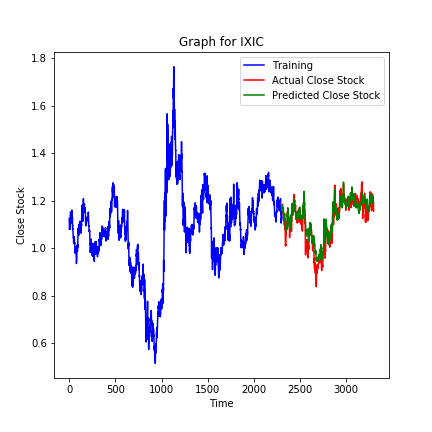
\includegraphics[width=\linewidth]{dnn.png}
    \caption{Expected vs Predicted for DNN} \label{fig:dnn_results}
\end{figure}
\FloatBarrier
\begin{figure}[ht]
\centering
    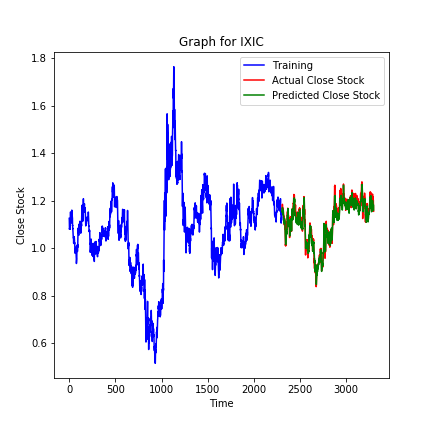
\includegraphics[width=\linewidth]{lstm.png}
    \caption{Expected vs Predicted for LSTM} \label{fig:lstm_results}
\end{figure}
\FloatBarrier

\FloatBarrier
\section{Discussion}

From this research, we have learned first-hand how truly complex the volatility of the stock market really is.
There is much more to learn on the subject and much more research needed to be done in order to create something that can be accurate enough to trust with financial investments.

The advancement of Neural Nets has opened the door to creating powerful predictive models that can intelligently sift through chaotic multivariate relationships, but much more training and know-how is required to perfect it.

Our models could be used as the starting point for future research and implementation.
Although our models failed to perform as well as desired, they could still be used as a springboard for future researchers in terms of data collection and preparation.

Our future research in this area will focus on how to improve our model results for LSTM and DNN.
Additionally, we implemented a DBN model for a single stock prediction but did not have time to adapt it to the newer benchmarking framework.
Thus our future research would hopefully also include completing the DBN model and comparing its performance to the other models.
We would also like to explore using deep learning for live stock market predictions in real time.

\bibliographystyle{IEEEtran}
\bibliography{references}
\end{document}
